\documentclass[a4paper]{article}
\usepackage[pdftex]{graphicx}
\usepackage[utf8]{inputenc}
\usepackage{enumerate}
\usepackage{siunitx}
\sisetup{locale=DE}
\usepackage{href-ul}
\hypersetup{
	colorlinks=true,
	linkcolor=blue,
	urlcolor=blue}
\usepackage{icomma}
\usepackage{colortbl}
\usepackage{multirow}
\usepackage{amssymb}
\usepackage{tikz}
\usetikzlibrary{positioning}
\usepackage{geometry}
\geometry{a4paper, top=15mm, left=15mm, right=15mm, bottom=15mm,
	headsep=10mm, footskip=12mm}

%Source: img_0243

% Start the document
\begin{document}
	%Title
	{\bf Parallel and Series Connection of Resistors}\\
	\begin{minipage}{0.5\textwidth}
		
		%Task 1
		You have the following resistors:\\ 2 x \fbox{$R=\SI{10}{\ohm}$}\\
		2 x \fbox{$R=\SI{33}{\ohm}$}\\
		2 x \fbox{$R=\SI{100}{\ohm}$}\\
		
		
	\end{minipage}
	\hfill
	\begin{minipage}{0.5\textwidth}
		
		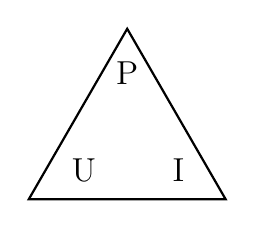
\begin{tikzpicture}[scale=1]
			% Triangle with side length 2.5 cm
			\coordinate (U) at (0,0); 
			\coordinate (I) at (2.5,0); 
			\coordinate (P) at (1.25, {2.5*sqrt(3)/2}); 
			
			% Draw lines
			\draw[thick] (U) -- (I) -- (P) -- cycle; 
			
			% Labeling inside
			\node[above=0.1cm of U, xshift=0.7cm] {\large U}; 
			\node[above=0.1cm of I, xshift=-0.6cm] {\large I};
		\node[below=0.3cm of P] {\large P};
	\end{tikzpicture}
	\hspace{3 cm}
	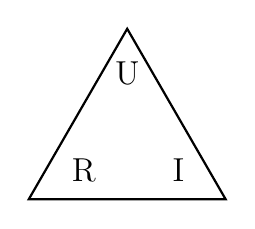
\begin{tikzpicture}[scale=1]
		% Triangle with side length 2.5 cm
		\coordinate (R) at (0,0); 
		\coordinate (I) at (2.5,0); 
		\coordinate (U) at (1.25, {2.5*sqrt(3)/2}); 
		
		% Draw lines
		\draw[thick] (R) -- (I) -- (U) -- cycle; 
		
		% Labeling inside
		\node[above=0.1cm of R, xshift=0.7cm] {\large R}; 
		\node[above=0.1cm of I, xshift=-0.6cm] {\large I}; 
		\node[below=0.3cm of U] {\large U};
	\end{tikzpicture}
\end{minipage}

\begin{enumerate}[1.]
	{\bf \item Connect each resistor to a 5V power source} and determine the current and the power. Which resistor has the highest power?
	
	 Enter the calculated and the measuerd values in the table!
	
	\begin{minipage}{0.5\textwidth}
		\item Series connection
		
		\renewcommand{\arraystretch}{2}
		\begin{tabular}{|>{\columncolor[gray]{.8}}p{1.5 cm}|p{1.5 cm}|p{1.5 cm}|p{1.5 cm}|}
			\hline
			\rowcolor[gray]{.8}	 $R_1 +R_2$ & $\SI{10}{\ohm}$	& $\SI{33}{\ohm}$	& $\SI{100}{\ohm}$	\\
			\hline
			\multirow{2}{*}{\vspace*{0.2cm}$\SI{10}{\ohm}$} 	& & & \\ \cline{2-4}
			& & & \\
			\hline
			\multirow{2}{*}{\vspace*{0.2cm}$\SI{33}{\ohm}$} 	& & & \\ \cline{2-4}
			& & & \\
			\hline
			\multirow{2}{*}{\vspace*{0.2cm}$\SI{100}{\ohm}$} 	& & & \\ \cline{2-4}
			& & & \\
			\hline
		\end{tabular}
	\end{minipage}
	\hfill
	\begin{minipage}{0.5\textwidth}
		\item Parallel connection
		
		\renewcommand{\arraystretch}{2}
		\begin{tabular}{|>{\columncolor[gray]{.8}}p{2 cm}|p{1.5 cm}|p{1.5 cm}|p{1.5 cm}|}
			\hline
			\rowcolor[gray]{.8}	 $\left(\frac{1}{R_1}+\frac{1}{R_2}\right)^{-1}$ & $\SI{10}{\ohm}$	& $\SI{33}{\ohm}$	& $\SI{100}{\ohm}$	\\
			\hline
			\multirow{2}{*}{\vspace*{0.2cm}$\SI{10}{\ohm}$} 	& & & \\ \cline{2-4}
			& & & \\
			\hline \multirow{2}{*}{\vspace*{0.2cm}$\SI{33}{\ohm}$} 	& & & \\ \cline{2-4}
			& & & \\
			\hline
			\multirow{2}{*}{\vspace*{0.2cm}$\SI{100}{\ohm}$} 	& & & \\ \cline{2-4}
			& & & \\
			\hline
		\end{tabular}
	\end{minipage}
	{\bf \item Which resistors do you connect to obtain the ...}\\
	
	\begin{enumerate}[a)]
		
		\hspace{-2 cm}
		\begin{minipage}{0.3\textwidth}
			\includegraphics[width=5 cm]{1wisch243.pdf}
		\end{minipage}
		\hspace{-0.5cm}
		\begin{minipage}{0.3\textwidth}
			\item ...largest total resistance?\\
			
			\renewcommand{\arraystretch}{2}
			\begin{tabular}{|>{\columncolor[gray]{.8}}p{1cm}|p{0.8cm}|p{0.8cm}|p{0.8cm}|p{0.8cm}|}
				\hline
				\rowcolor[gray]{.8}	  & $R$ & $U$	& $I$	 & $P$\\
				\hline
				1 & & &  & \\
				\hline
				2	& & &  & \\
				\hline
				3 & & &  & \\
				\hline
				Total & & $\SI{5,0}{\volt}$&  & \\
				\hline
			\end{tabular}
		\end{minipage}
		\hspace{1cm}
		\begin{minipage}{0.3\textwidth}
			\item ...smallest total resistance?\\
			
			\renewcommand{\arraystretch}{2}
			\begin{tabular}{|>{\columncolor[gray]{.8}}p{1cm}|p{0.8cm}|p{0.8cm}|p{0.8cm}|p{0.8cm}|}
				\hline
				\rowcolor[gray]{.8}	  & $R$ & $U$	& $I$	 & $P$ \\
				\hline
				1 & & &  & \\
				\hline 2	& & &  & \\
				\hline
				3 & & &  & \\
				\hline
				Total & & $\SI{5.0}{\volt}$&  & \\
				\hline
			\end{tabular}
		\end{minipage}
		
		\hspace{-2 cm}
		\begin{minipage}{0.3\textwidth}
			\includegraphics[width=5 cm]{2wisch243.pdf}
		\end{minipage}
		\hspace{-0.5cm}
		\begin{minipage}{0.3\textwidth}
			\item ...largest total resistance?
			
			\renewcommand{\arraystretch}{2}
			\begin{tabular}{|>{\columncolor[gray]{.8}}p{1cm}|p{0.8cm}|p{0.8cm}|p{0.8cm}|p{0.8cm}|}
				\hline
				\rowcolor[gray]{.8}	  & $R$ & $U$	& $I$	 & $P$ \\
				\hline
				1 & & &  & \\
				\hline
				2	& & &  & \\
				\hline
				3 & & &  & \\
				\hline
				Total & & $\SI{5.0}{\volt}$&  & \\
				\hline
			\end{tabular}
		\end{minipage}
		\hspace{1cm}
		\begin{minipage}{0.3\textwidth}
			\item ...smallest total resistance?\\
			
			\renewcommand{\arraystretch}{2}
			\begin{tabular}{|>{\columncolor[gray]{.8}}p{1cm}|p{0.8cm}|p{0.8cm}|p{0.8cm}|p{0.8cm}|}
				\hline
				\rowcolor[gray]{.8}	  & $R$ & $U$	& $I$	 & $P$ \\
				\hline
				1 & & &  & \\
				\hline
				2	& & &  & \\
				\hline
				3 & & &  & \\
				\hline
				Total & & $\SI{5,0}{\volt}$&  & \\
				\hline
			\end{tabular}
			\end{minipage}
			
			
		\end{enumerate}
	

\end{enumerate}

\fbox{
\begin{minipage}{0.5\textwidth}
For the solution, please click \href{https://www.okuyakl.de/phys/p8wipareiL243/le243.pdf}{here} or scan the QR code.\\
Further worksheets are available at

\href{https://www.okuyakl.de}{www.okuyakl.de}
\end{minipage}
\hfill
\begin{minipage}{0.4\textwidth}  \includegraphics[width=1.5 cm]{../../viecher/zwe03} 
\includegraphics[width=3 cm]{qre243} 
\includegraphics[width=2 cm]{../../viecher/afanticon1} 

\end{minipage}}
\end{document}